
\graphicspath{ {mainmatter/Verplank_2002/} }
\title*{2002: The Plank: Designing a Simple Haptic Controller}
\titlerunning{A Simple Haptic Controller}

\author{Bill Verplank, Michael Gurevich and Max Mathews}
\authorrunning{Verplank et al.}

%\institute{Bill Verplank \at Center for Computer Research in Music and Acoustics, Stanford University, Stanford, California, USA \email{bill@billverplank.com} 
%\and Michael Gurevich \at University of Michigan, School of Music, Theatre \& Dance, Ann Arbor, Michigan, USA \\ \email{mdgurev@umich.edu} \\ Affiliation at time of original publication: Center for Computer Research in Music and Acoustics, Stanford University, Stanford, California, USA
%\and Max Mathews \at Center for Computer Research in Music and Acoustics, Stanford University, Stanford, California, USA}
%
% Use the package ''url.sty'' to avoid
% problems with special characters
% used in your e-mail or web address
%
\maketitle

\abstract*{Active force-feedback holds the potential for precise and rapid controls. A high performance device can be built from a surplus disk drive and controlled from an inex- pensive microcontroller. Our new design,The Plank has only one axis of force-feedback with limited range of motion. It is being used to explore methods of feeling and directly manipulating sound waves and spectra suitable for live performance of computer music.}

\section{Introduction}

In 1996, Perry Cook at Princeton, Ben Knapp at San Jose State and Chris Chafe at Stanford University started teaching a video-linked course in human-computer interaction technology. Max Mathews and Bill Verplank have in the last two years focussed the course on music controllers \cite{Verplank:2001} for the masters program in music science and technology. At CCRMA, we have a Phantom, a high-performance three-degree-of-freedom force-feedback device donated by Interval Research. We want a simpler device for experimentation and performance.

\begin{figure}[ht]
% Use the relevant command for your figure-insertion program
% to insert the figure file.
% For example, with the graphicx style use
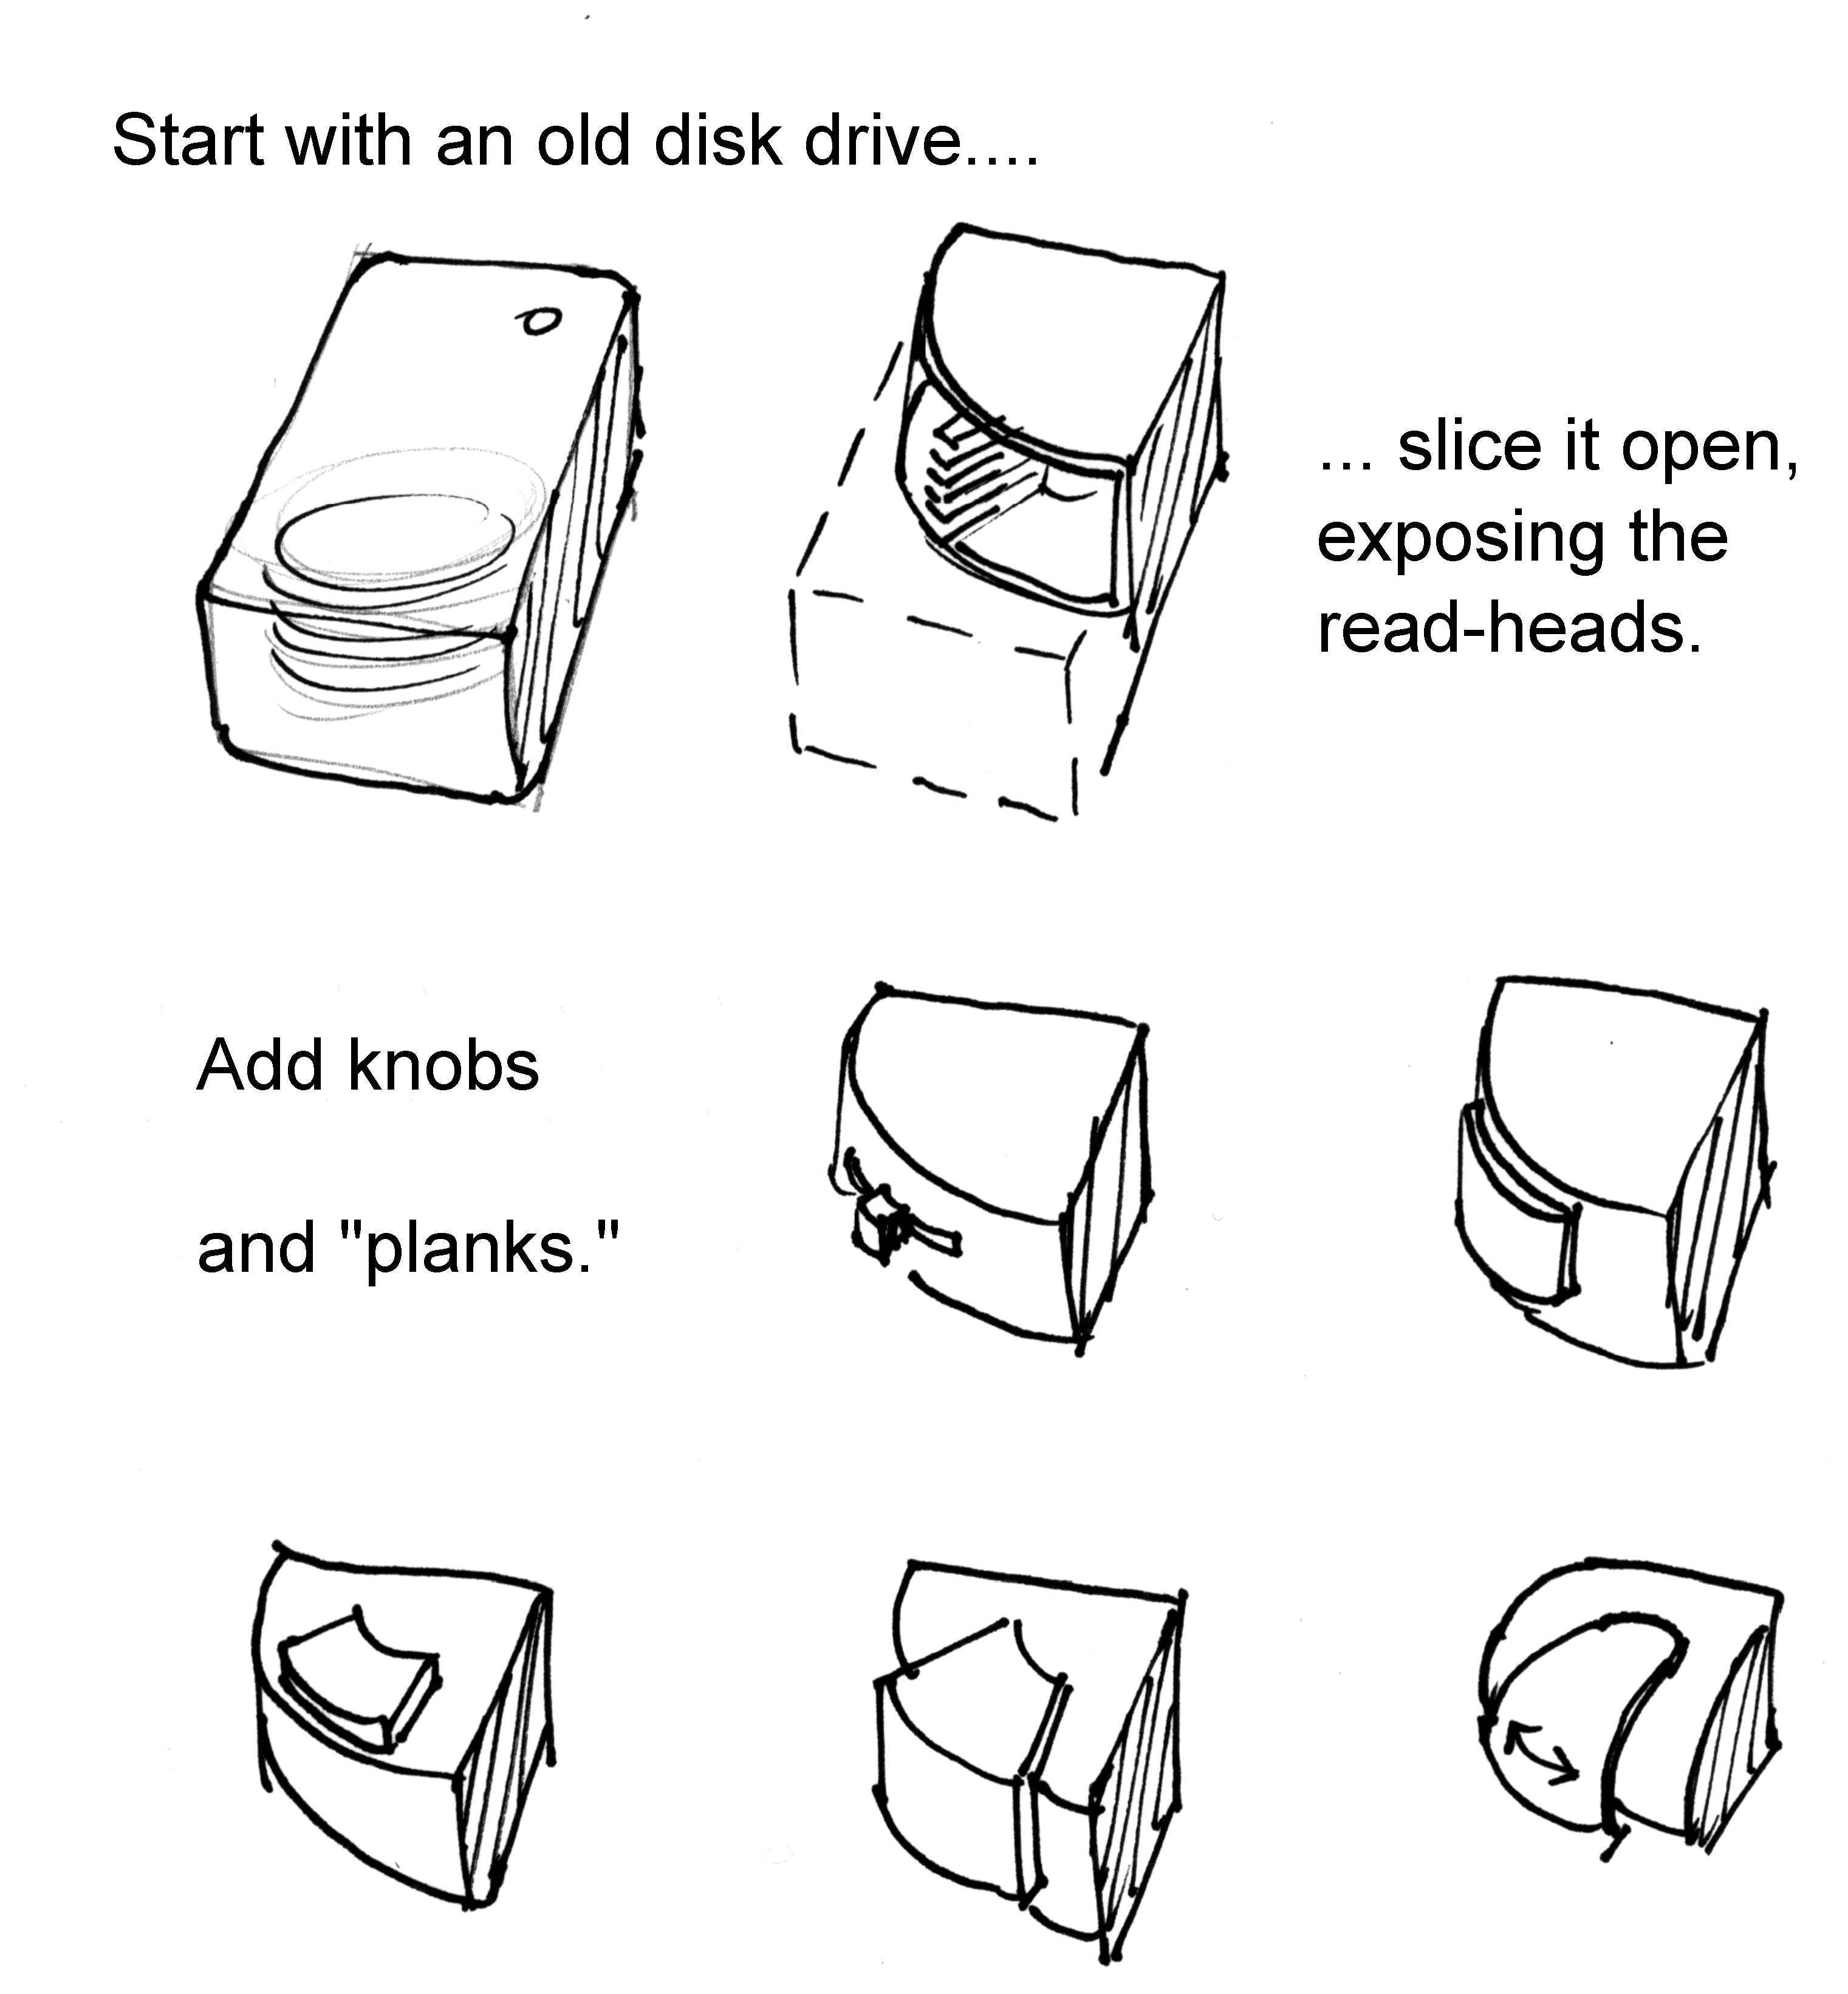
\includegraphics[width=9cm]{Plank1}
\centering

% If no graphics program available, insert a blank space i.e. use
%\picplace{5cm}{2cm} % Give the correct figure height and width in cm
%
\caption{The Plank concept}
\label{Verplank:fig:1}       % Give a unique label
\end{figure}


\subsection{Scanned Synthesis}
\label{Verplank:sub:1_1}
At Interval, we used Phantoms \cite{Massie:1994} to explore the value of force-feedback. One discovery was that simple spring-mass simulations, which are uncontrollable without force-feedback, can be controlled simply by letting the vibrating system transfer energy to the human. In feeling a simulated wave, Verplank, Shaw and Mathews had the idea of listening to the shapes. This came to be known as ``scanned synthesis'' \cite{Verplank:2000}. The idea is to directly manipulate a dynamic wave shape at human-hand frequencies while scanning the wave shape out at audio frequencies. The pitch is determined by the length of the wave and the scan rate. The timbre is determined by the wave shape which is being continuously controlled by the performer.

\subsection{Haptics}
\label{Verplank:sub:1_2}
The term haptics is used by psychologists to describe the human sense of touch including skin senses as well as muscle and joint senses. Recently, ``haptic'' devices have made it to market in vibrating pagers, rumble-packs, force-feedback joysticks, steering wheels and mice. There are active research communities and a small industry building devices. Standards have been established for communication and development. At Interval, we explored the potential for simple haptic devices for media control and expression \cite{Snibbe:2001}.

\section{Haptic Illusions}

The Plank is designed to take advantage of several illusions that allow us to reduce the device complexity while maintaining haptic fidelity. The key feature is a surface which measures forces orthogonal to its motion. With a measured surface force, the Plank simulates terrain as well as friction and dynamics.

\subsection{Slope}
\label{Verplank:sub:2_1}
When you press down on a surface, it usually pushes back on you with a ``surface normal'' perpendicular to the surface. The forces fed back by the device can give the illusion of slopes of a surface. Small variations in force as you move along the surface are felt as bumps. In a pioneering study, Margaret Minsky explored this phenomenon of simulated textures with a two-degree-of-freedom force-feedback joystick \cite{Minsky:1995}. The Plank reinforces this illusion by measuring the force applied by the user normal to the motion and making the tangential force-feedback proportional.

\begin{figure}[ht]
% Use the relevant command for your figure-insertion program
% to insert the figure file.
% For example, with the graphicx style use
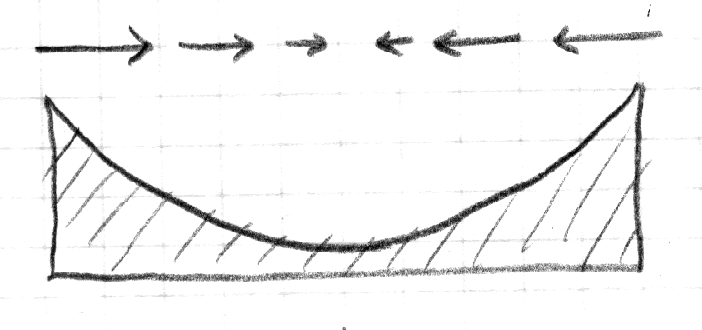
\includegraphics[width=5cm]{Plank2}
\centering

% If no graphics program available, insert a blank space i.e. use
%\picplace{5cm}{2cm} % Give the correct figure height and width in cm
%
\caption{Slope illusion}
\label{Verplank:fig:2}       % Give a unique label
\end{figure}

\subsection{Clutch}
\label{Verplank:sub:2_2}
Rob Shaw simulated a variety of dynamic systems which could be engaged by applying forces \cite{Snibbe:2001}. We came to call this phenomenon the ``haptic clutch.'' By pressing on The Plank, you engage with a simulated moving object. This technique compensates for the limited travel of The Plank and allows the illusion of wide reach.

\begin{figure}[ht]
\centering
% Use the relevant command for your figure-insertion program
% to insert the figure file.
% For example, with the graphicx style use
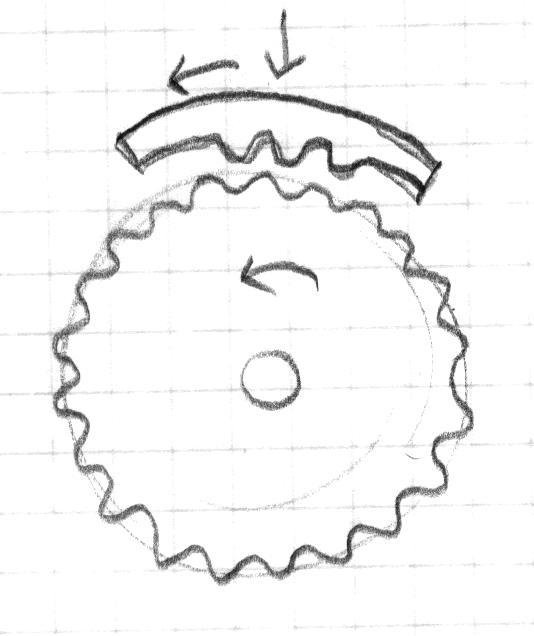
\includegraphics[width=5cm]{Plank3}
%
% If no graphics program available, insert a blank space i.e. use
%\picplace{5cm}{2cm} % Give the correct figure height and width in cm
%
\caption{The haptic clutch}
\label{Verplank:fig:3}       % Give a unique label
\end{figure}

\section{Hardware}

The construction of The Plank was undertaken as an educational exercise using inexpensive or found components. It is described in some detail with the hope that others will take on such do-it-yourself haptics.

\begin{figure}[ht]
\centering

% Use the relevant command for your figure-insertion program
% to insert the figure file.
% For example, with the graphicx style use
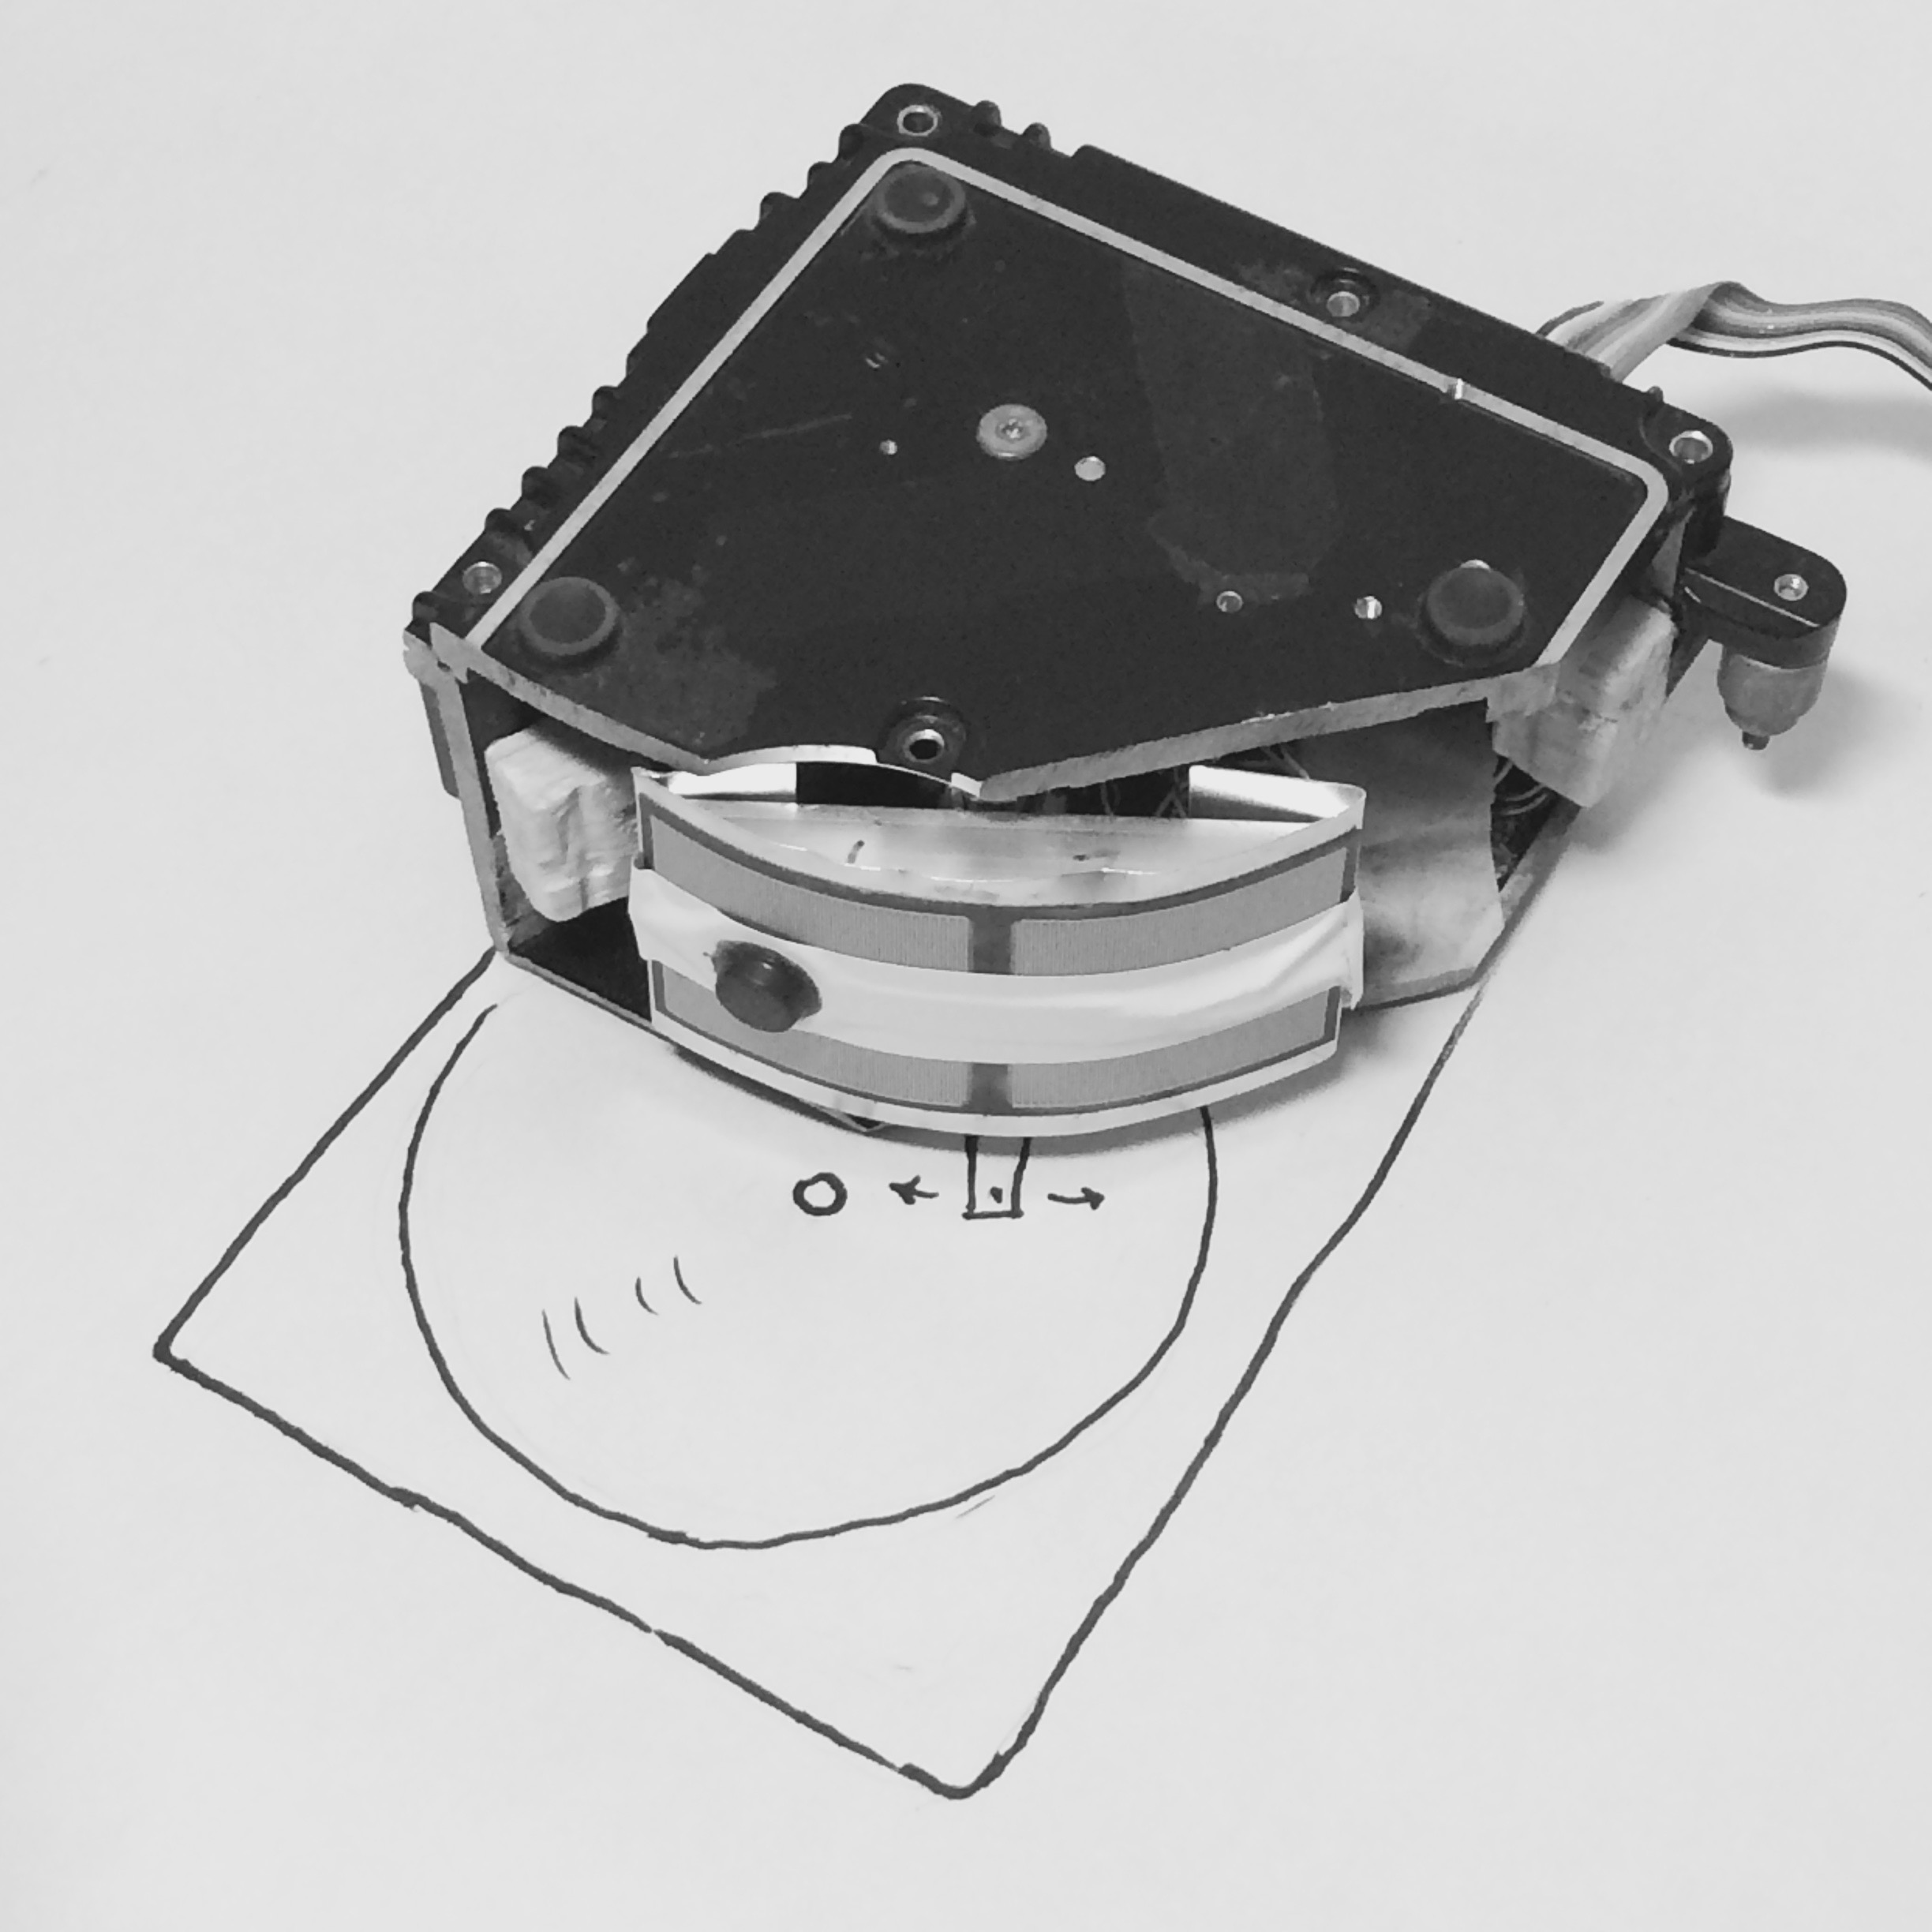
\includegraphics[width=11.3cm]{Plank4}
%
% If no graphics program available, insert a blank space i.e. use
%\picplace{5cm}{2cm} % Give the correct figure height and width in cm
%
\caption{Disk drive cutaway}
\label{Verplank:fig:4}       % Give a unique label
\end{figure}


\subsection{Motors}

Rotary DC motors are the most common actuators used for haptic display from \$1 vibrators to \$100 joysticks to \$10,000 Phantoms. In contrast, the motors chosen for The Plank are from computer disk drives where they position the read-heads. They are known as voice-coil motors. There is no requirement for gears or pulleys, both the drive and the sensor are directly coupled to the motor. Several haptic displays have been made from disk drive motors. Hong Tan studied tactile communication bandwidth with three independent disk-drive motors \cite{Tan:1996}. Pietro Buttolo built a planar mechanism for positioning the tip of a stylus using three disk-drive motors \cite{Buttolo:1995}. The voice coil motors are readily available as castoffs in crashed disks.

\subsection{Microcontroller}
\label{Verplank:sub:3_2}
To ensure rapid computation of the forces, an Atmel mega163 microcontroller is dedicated to local control of The Plank. % \cite{Atmel:}. 
It operates at up to 8 Mhz with 8 channels of 10-bit A/D ($\sim$10k samples/second), 32 I/0 ports, 16K bytes of program memory and 1024 bytes of data memory. The microcontroller has a UART for communication via MIDI with a synthesizer or real-time DSP software. Interrupts keep the sampling, or servo update at a steady rate up to 4kHz.

\subsection{Sensing and orthogonal force control}
\label{Verplank:sub:3_3}
A hall-effect sensor is used for rotary position feedback read by an 10-bit A/D converter built into the microcontroller. A 12-bit DAC commands a power op-amp for generating up to 3A current and forces up to 5 Newtons ($\sim$1 lb) at the finger tips (for short times). The sensing and power amp came from the design for a simple device used in teaching haptics \cite{Richard:1997}. Force sensitive resistors measure finger pressure on the surface of The Plank.

\begin{figure}[ht]
\centering

% Use the relevant command for your figure-insertion program
% to insert the figure file.
% For example, with the graphicx style use
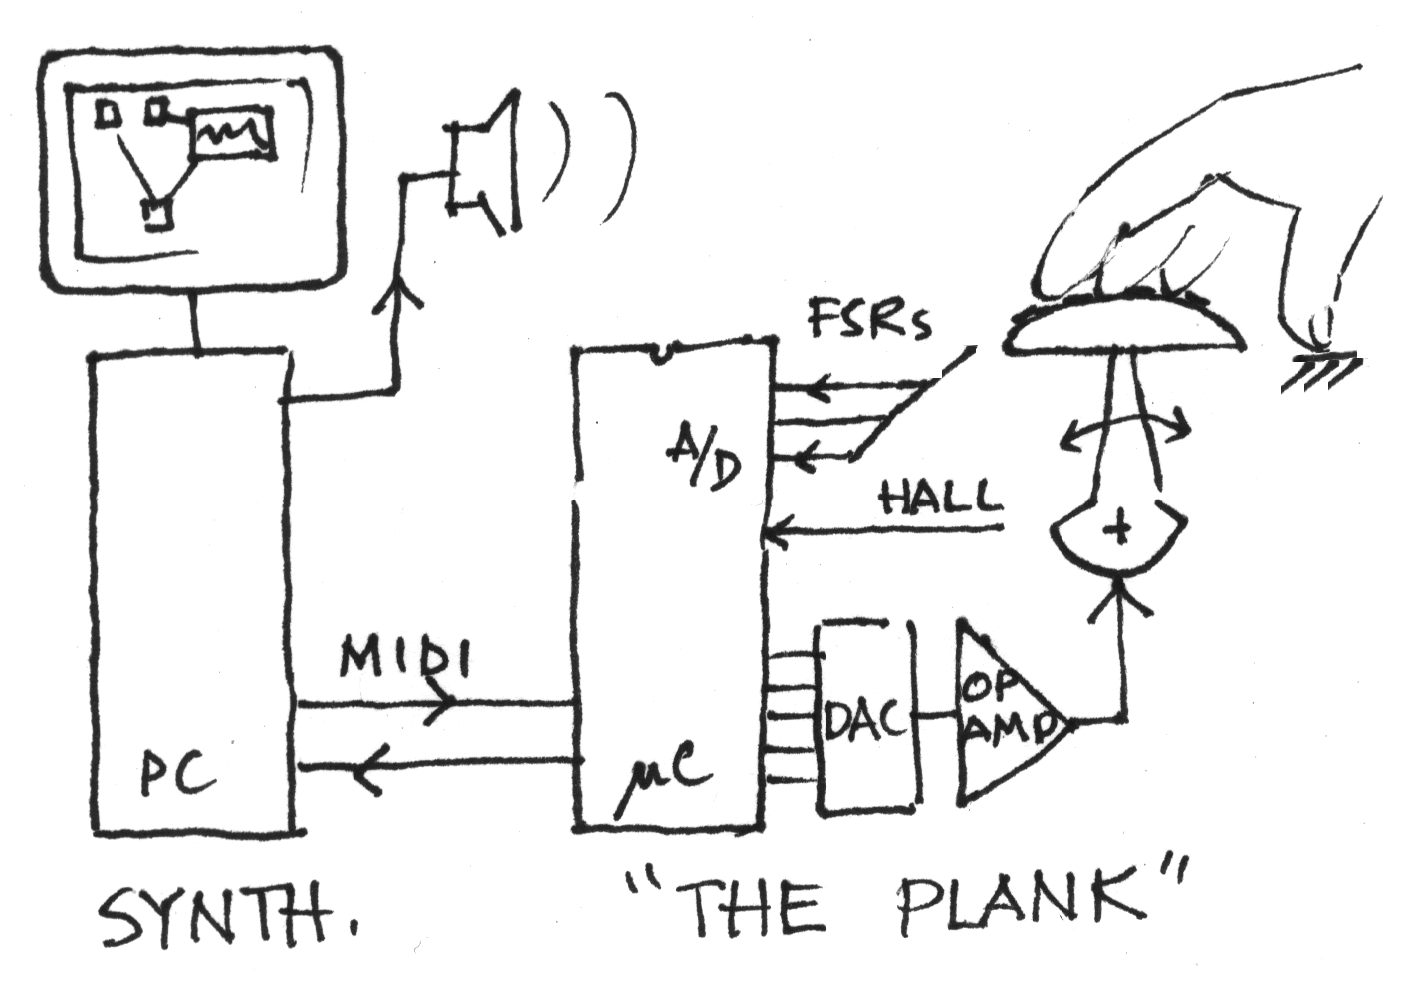
\includegraphics[width=11.3cm]{Plank5}
%
% If no graphics program available, insert a blank space i.e. use
%\picplace{5cm}{2cm} % Give the correct figure height and width in cm
%
\caption{System diagram}
\label{Verplank:fig:5}       % Give a unique label
\end{figure}

\section{Effects}

\subsection{Table of Forces: Terrain}
\label{Verplank:sub:4_1}
The microprocessor holds a small look-up table with a force for every measured position of The Plank. In scanned synthesis, the shape represents one cycle of a wave or piece of terrain. As you move The Plank, you feel the shape of the terrain; when you apply pressure, you can manipulate the terrain.


\begin{figure}[ht]
\centering

% Use the relevant command for your figure-insertion program
% to insert the figure file.
% For example, with the graphicx style use
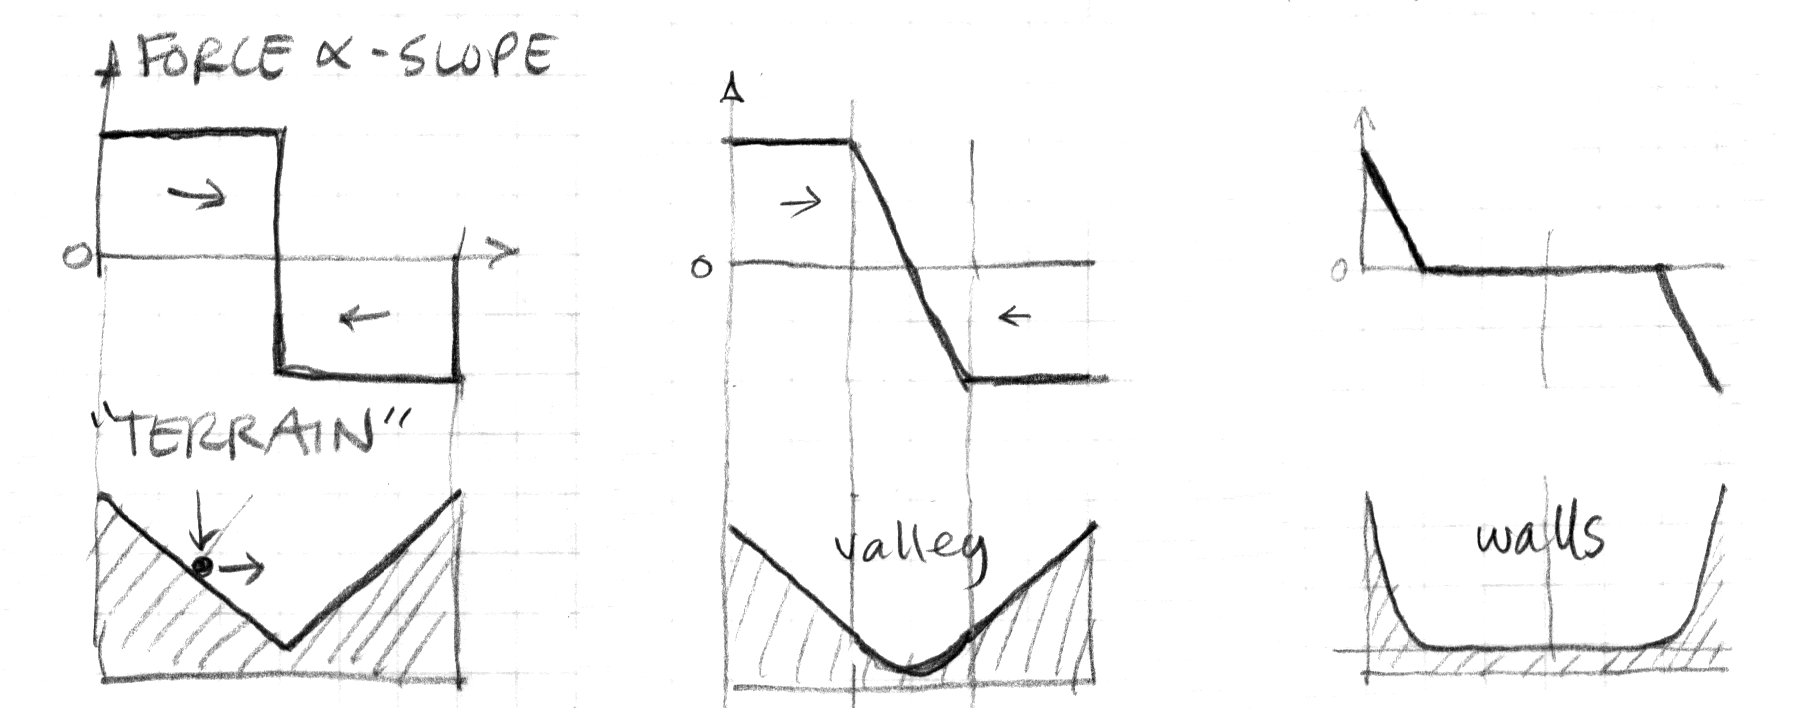
\includegraphics[width=11.3cm]{Plank6}
%
% If no graphics program available, insert a blank space i.e. use
%\picplace{5cm}{2cm} % Give the correct figure height and width in cm
%
\caption{Forces create terrain illusions}
\label{Verplank:fig:plank6}       % Give a unique label
\end{figure}

\subsection{Motion: Dynamics}

The whole terrain can be moved left or right (actually just a pointer into the table). Buffers can extend the table beyond the range of Plank motion (in the case of scanned synthesis, the table is circular and the buffers are not necessary). To simulate a single mass attached to a spring, one detent or deep valley in the terrain represents the position of the mass, its slopes represent the stiffness of the spring. The force on The Plank increases as it moves ``up the slope of the valley.'' The acceleration of the mass is simply computed from the force being fed back to The Plank.

\subsection{Friction}

We have experimented using the Phantom with several friction models. The simplest is ``stick-slip,'' Just one spring that builds up to a maximum and then ``breaks'' feels like plucking a string. When one spring breaks another can grab hold; many small ones make a fine texture that makes it easy to hold still. It is easy to add ``viscosity'' by measuring velocity and resisting the motion proportionately.
Combinations of these effects should be able to provide a wide variety of behaviors. Examples are shown in Table 1.

\begin{table}
\label{Verplank:tab:1} 
\centering
\ra{1.3}
\caption{The Plank's effects combined}
\vspace{3pt} \noindent
\begin{tabular}{llll}
\toprule
\textbf{Effect} & \textbf{Terrain} & \textbf{Dynamics} & \textbf{Friction}  \\
\midrule  
DETENTS  & Valleys  \hspace{2cm}  & --   & --\\
PLATTER & None cleavage & Inertia \hspace{2cm} & Stick-slip\\
WAVE \hspace{2cm} & Shape  & Mass/Spring & Viscosity\\
PLUCK & --  & String & Stick-slip\\
\bottomrule
\end{tabular}
\end{table}

\begin{figure}[ht]
\centering
% Use the relevant command for your figure-insertion program
% to insert the figure file.
% For example, with the graphicx style use
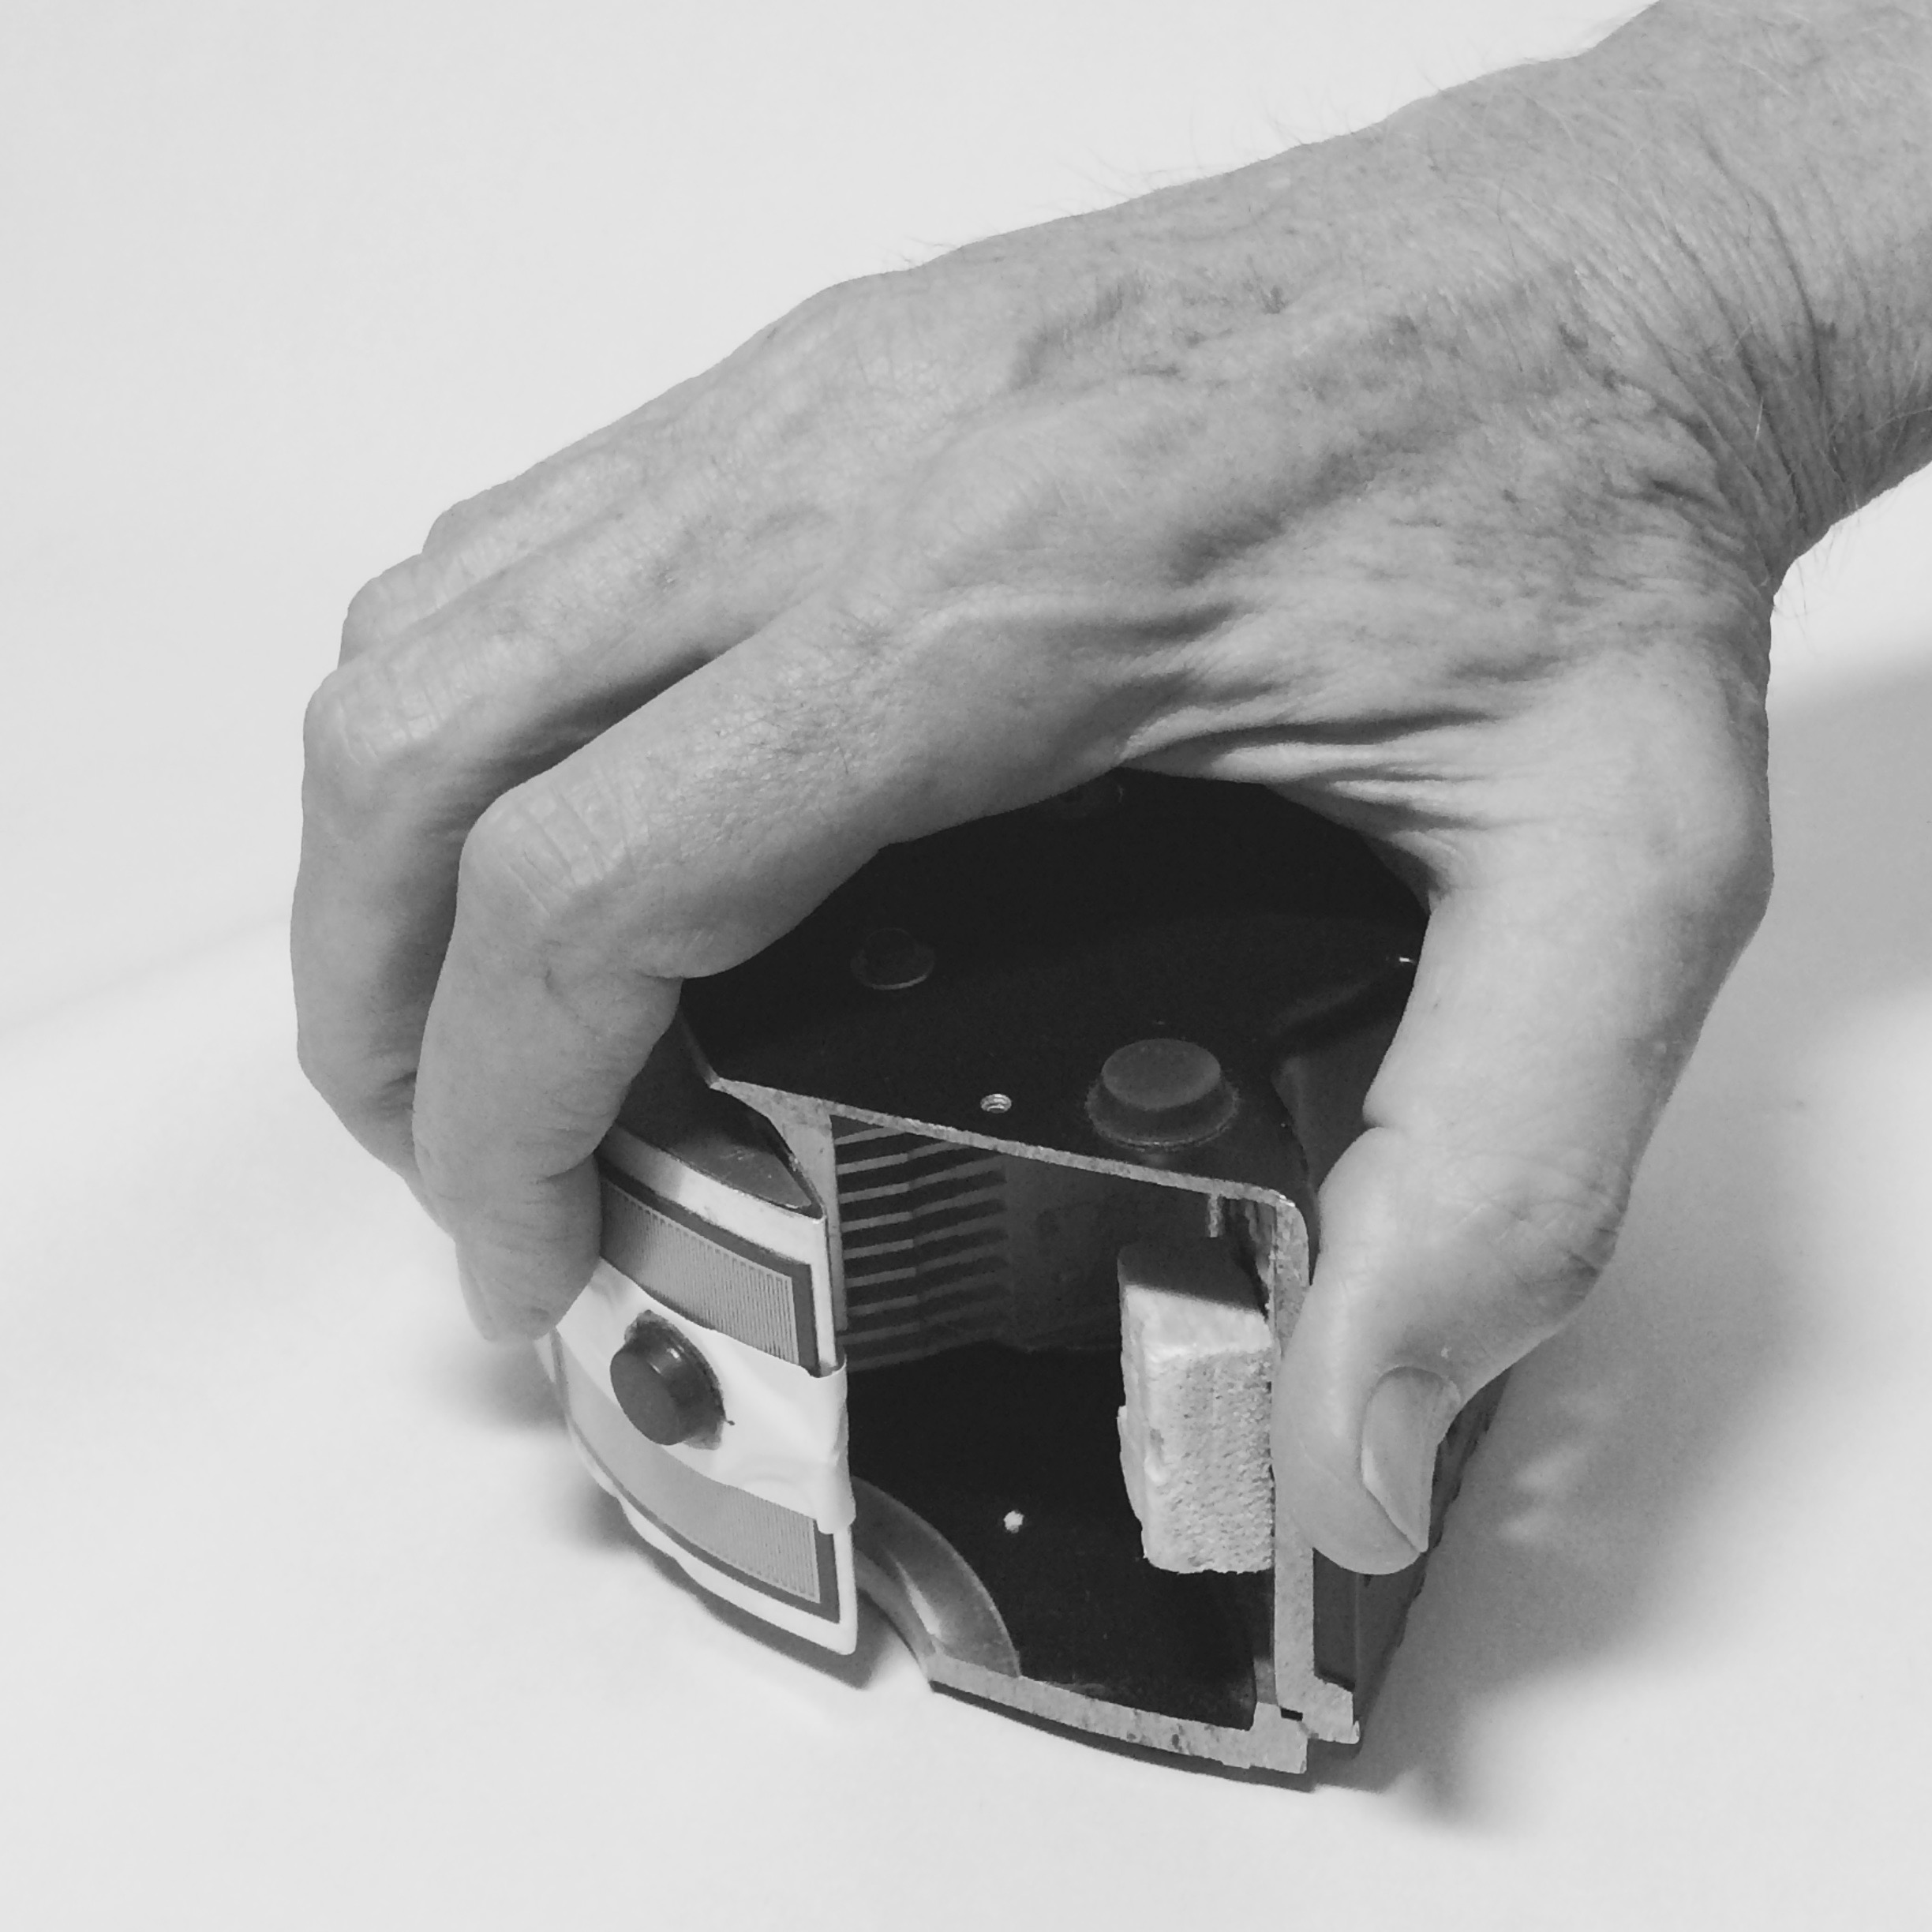
\includegraphics[width=3.85cm]{Plank7a}
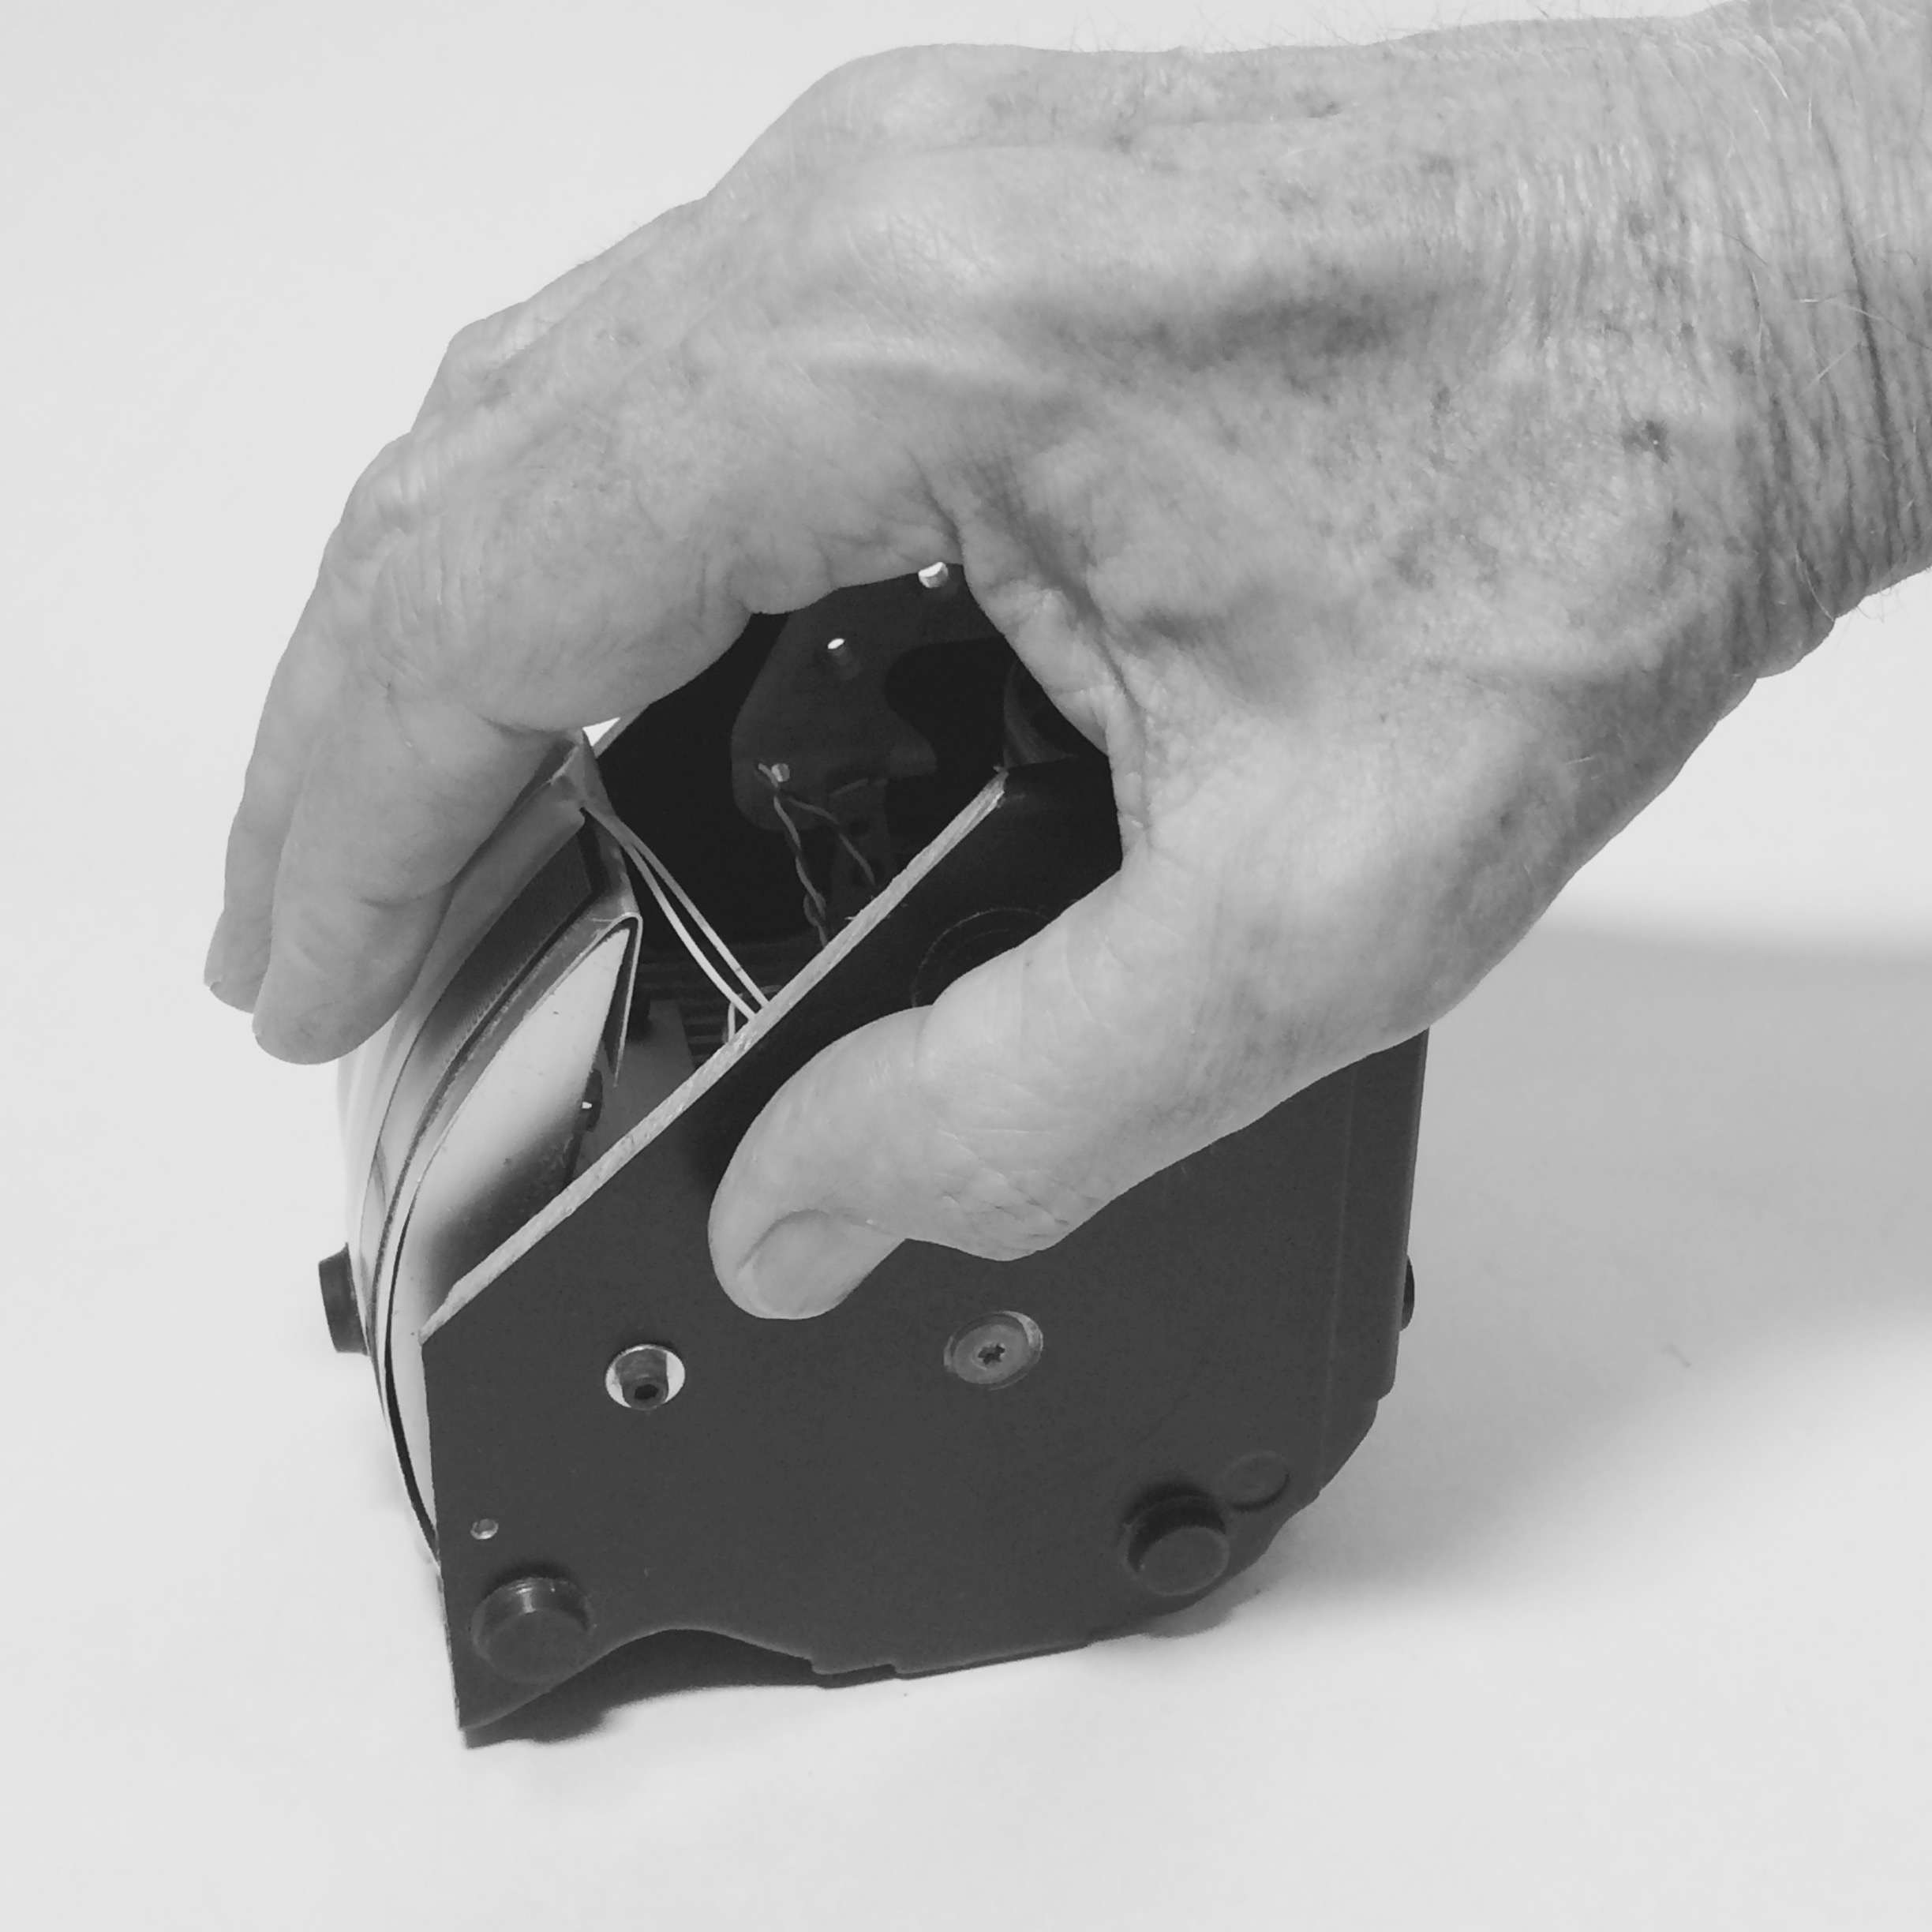
\includegraphics[width=3.85cm]{Plank7b}
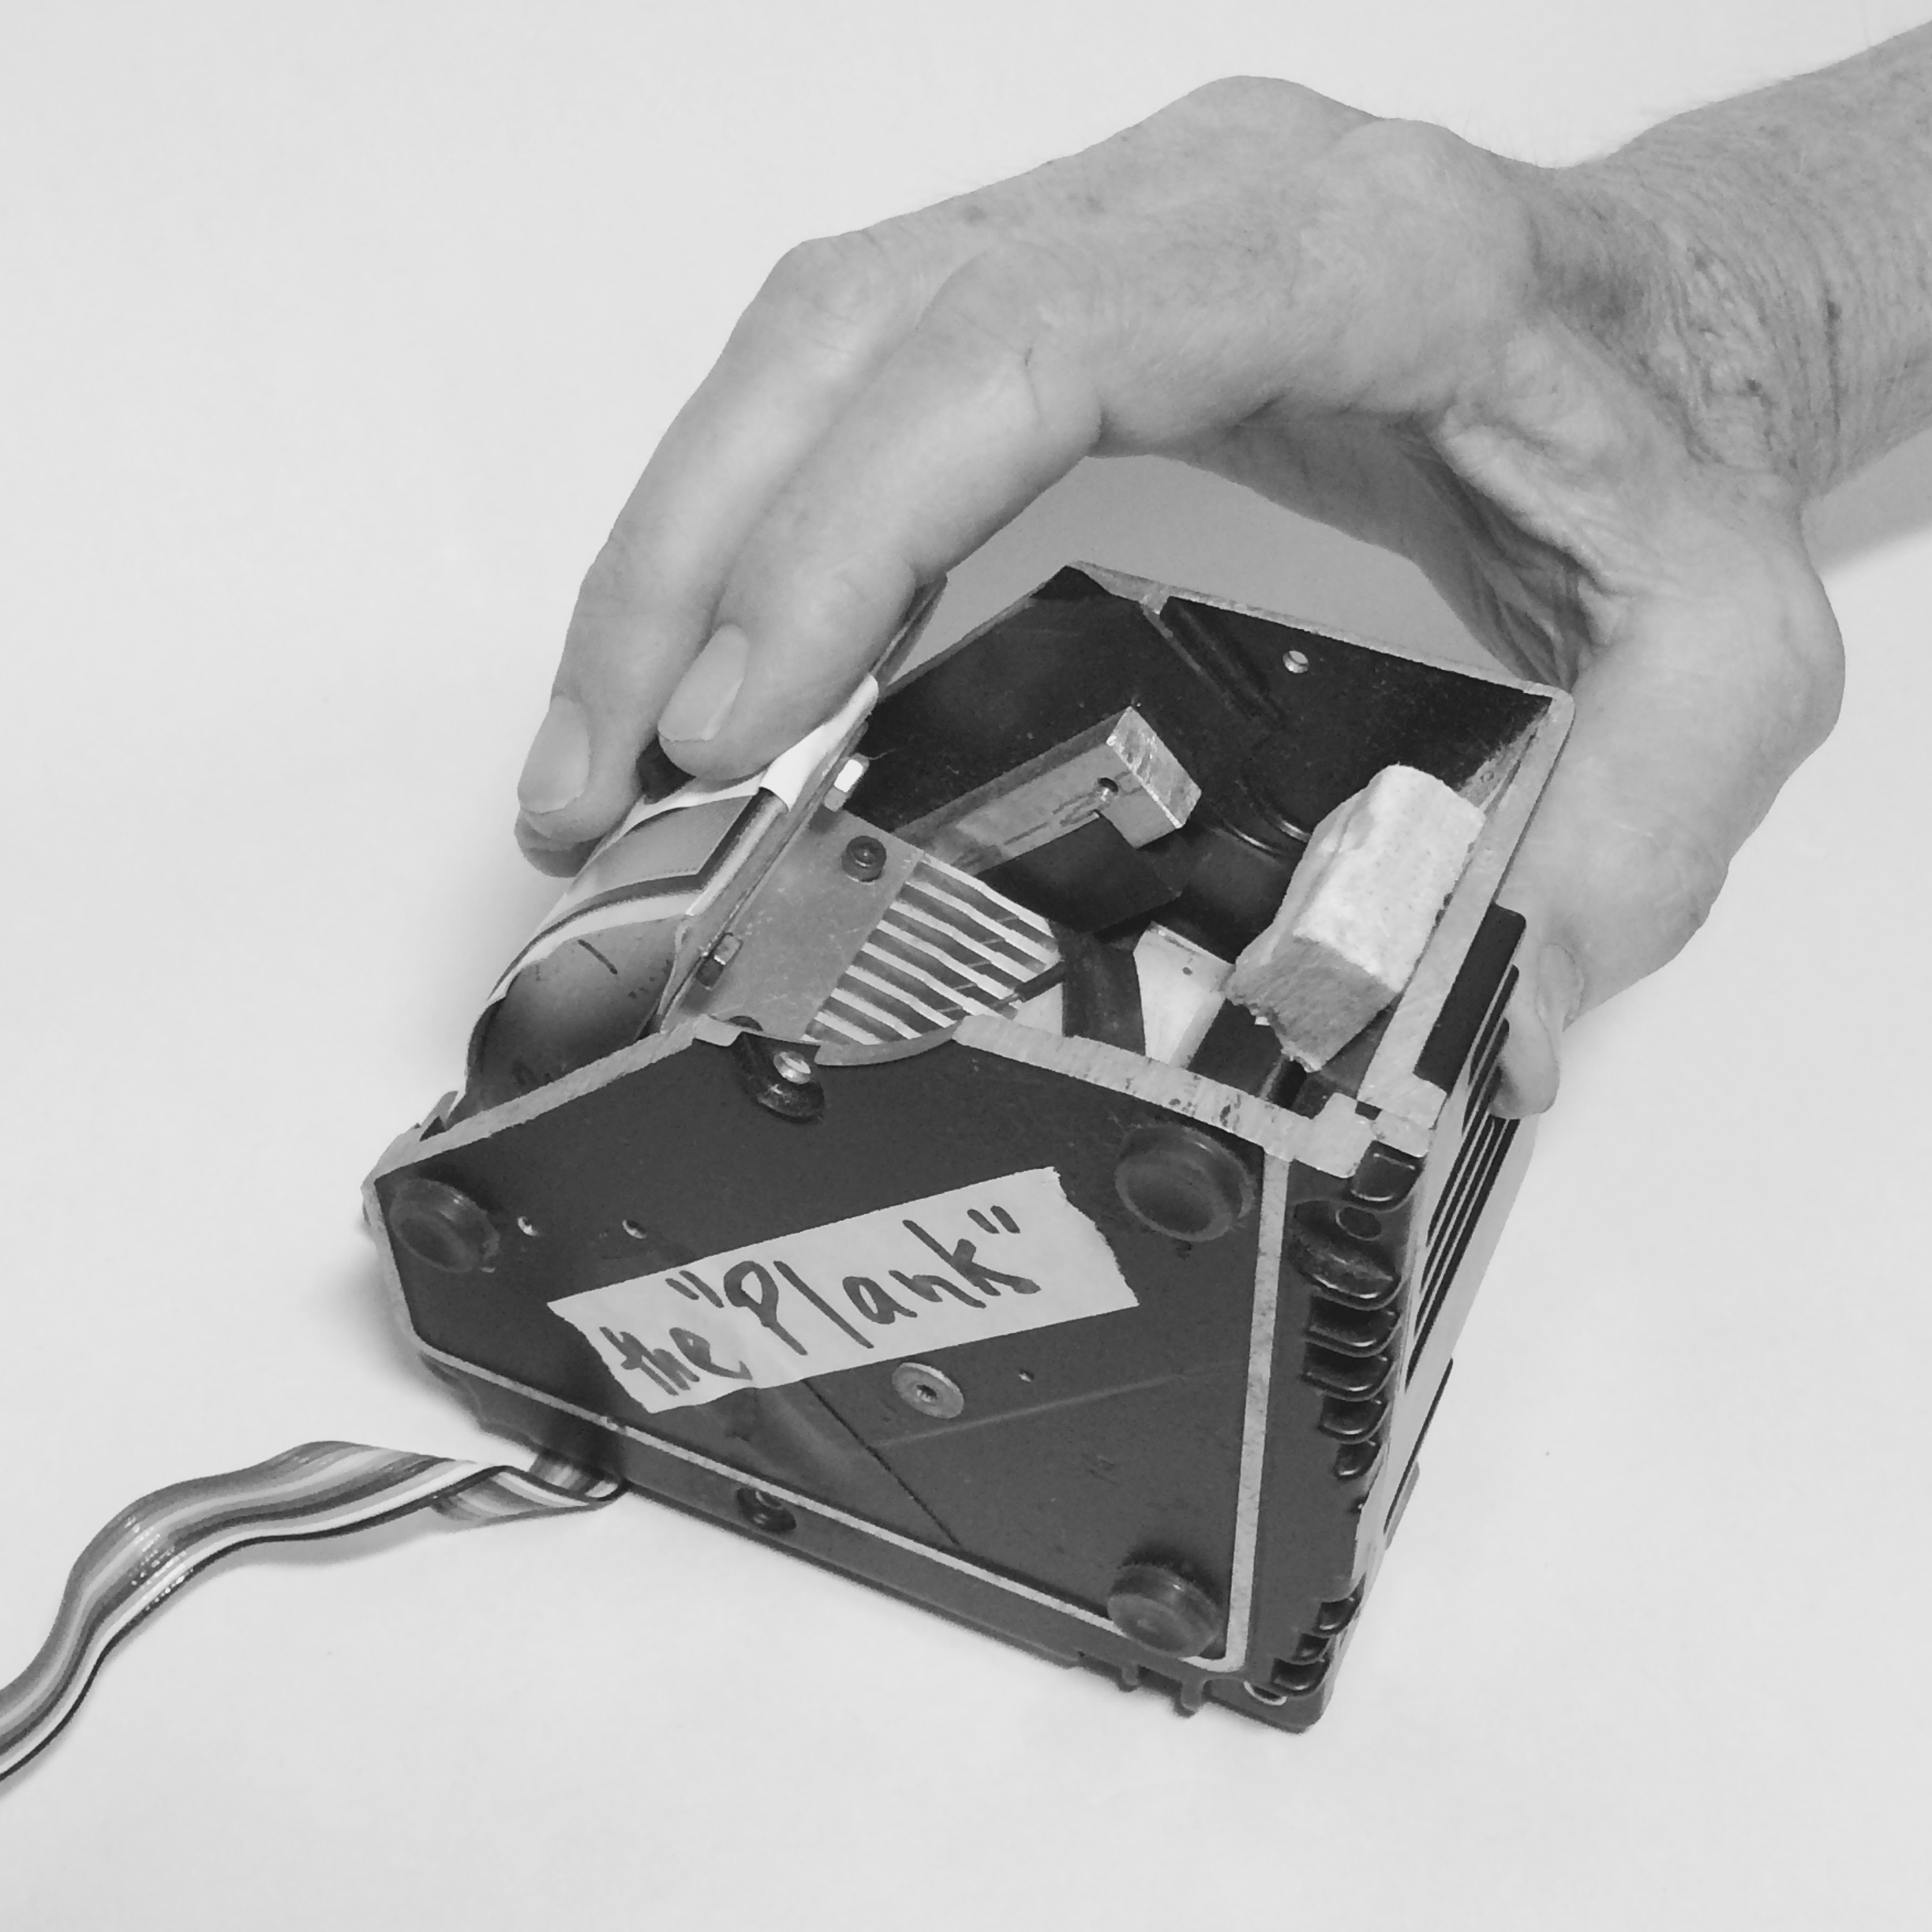
\includegraphics[width=3.85cm]{Plank7c}
\caption{Hand positions}
\label{Verplank:fig:7}       % Give a unique label
\end{figure}

\section{Progress and Plans}

The hardware and microprocessor software are working in a rough prototype. We are not yet communicating with the synthesizer let alone producing music. The Plank will be used to interface with scanned synthesis, and we will explore mappings of The Plank's interactions with wave terrains to audio parameters. An advantage of haptic interfaces for real-time music performance is that the performer now has another direct bidirectional interaction with the sound through his or her hands. We anticipate being able to simulate the feel of some traditional musical instruments (drums, piano, strings) allowing precise and fast control. We are also looking for new effects and unexpected, expressive sounds.

\begin{acknowledgement}
Interval Research supported six years of haptics research. Margaret Minsky, Brent Gillespie, Sile O'Modhrain, and in particular Karon Maclean inspired our work on simple devices. Rob Shaw showed us the magic of dynamics and helped invent scanned synthesis. Chris Chafe gave us a home at CCRMA.
\end{acknowledgement}

\section*{Author Commentary: Personal Reflections on The Plank}
\paragraph{Michael Gurevich and Bill Verplank}

The Plank was a direct outgrowth of research and experimentation by Verplank and Mathews at Interval Research that was in many ways a prototype for NIME itself: we were interested in developing new, interactive, audiovisual hardware/software technologies with primarily open-ended, creative applications.

The project can also be seen as an extension of Max Mathews' vision for computer music evident in his first real-time interactive computer music system---GROOVE---and ultimately of course in his Radio Baton. Max was an amateur violinist, but he didn't think the computer would make him a better musician. At Bell Labs, Max was among the pioneers to use the computer as a tool for simulation---initially to simulate telephone transmission systems; elaborating on this premise, he thought the computer could allow him (or anyone else) to simulate the experience of a great musician. Of course, there are many kinds of musical experiences, each of which is multi-faceted, and it ultimately occurred to Max and others that one aspect that was missing in many digital music systems was feel: the tactile, tangible relationship a performer has with their instrument; the ways an instrument pushes back on you when you push on it.

Others had certainly explored the intersection of haptics and music before The Plank. Brent Gillespie and Sile O'Modhrain preceded us at CCRMA \cite{Gillespie:1995}, and Claude Cadoz's group had been working on the problem since at least 1978 \cite{Cadoz:2003}. Charles Nichols presented his sophisticated haptic vBow at the same NIME (2002) as The Plank.  But in what we feel would become the essential spirit of NIME, and indeed the nascent ``Maker'' movement, The Plank sought to make haptics ``easy;'' the paper was really intended as a catalyst for others to try the same thing. It employed easily-obtainable, inexpensive, and largely open-source tools, and emphasized that the underlying principles could be implemented with little effort. 

It is worth noting that The Plank marked the first documented use in NIME of an Atmel AVR microcontroller (for which we owe an eternal debt of gratitude to Pascal Stang), which would become the core of the Arduino, now probably the most popular development board for physical computing in the world that powers much ``making'' and much of NIME.  As it turns out, this is no accident: Bill Verplank brought Pascal Stang's AVRmini development boards and AVRLib library (as well as The Plank) to the Interaction Design Institute Ivrea; when Massimo Banzi and others were frustrated they couldn't easily get their hands on more AVRmini boards, Arduino was born. 

One of the perpetual problems with experiential phenomena such as music is the difficulty in communication around the experience through the written medium. We are fortunate with music both to have a centuries-old discourse to draw upon, but also that it is relatively easy today to embed and distribute audio alongside or within written forums. We do not have either of these luxuries with haptics; for now, the best way to communicate about haptics, as well as to generate interest in musical haptics, is to ``feel it.'' For this reason, Verplank has remained committed to conducting courses and workshops on music and haptics, and to elaborating on making accessible tools like The Plank readily available. These efforts include a  ``Music \& Motors'' workshop that has run at the Copenhagen Institute of Interaction Design since 2011, which has produced numerous inventive projects, as well as a dedicated development board built on the Teensy 3.1 platform \cite{Bak:2015}. Several alumni of our workshops and courses have not only made substantial subsequent contributions at the intersection of music and haptics (e.g. \cite{Gillespie:1995}), but have also been responsible for expanding the incorporation of haptics into consumer products at companies including Apple and Immersion. 

Haptics remains a vital topic at NIME. Bill Verplank has continued to develop The Plank with a similar emphasis on helping to understand and emulate the ``feel'' of playing an acoustic instrument. Some of the most exciting work on haptics in NIME has come from Edgar Berdahl, who fulfilled one of our initial objectives for The Plank by creating a direct haptic interface to a computational acoustic simulation of a musical instrument---effectively unifying the haptic and sound synthesis models \cite{Berdahl:2009}. Berdahl has also expanded on O'Modhrain's work to examine ways that active force feedback may improve musicians' abilities to perform with digital and electroacoustic instruments \cite{Berdahl:2009a}. 

\section*{Expert Commentary: Haptics for Sonic Interaction Design using Recycled Motors}
\paragraph{Edgar Berdahl}

%\input{referenc}

Bill Verplank was a pioneer of NIME even before NIME became a recognized field. In the mid-1980s, he co-coined the term interaction design, and he helped introduce interaction design into digital musical practice by leading the NIME course at Stanford University for many years \cite{Berdahl:2013a}. He introduced valuable concepts to the NIME community such as distinguishing between musical ``buttons'' and musical ``handles,'' sketching and critiquing project ideas using his Interaction Design Framework, and designing haptic controls for music, which is the subject of this commentary.

In their seminal paper, Bill Verplank et al. described the first work on enabling students in a NIME course to experiment with haptic force-feedback controls. This work included the development of The Plank haptic device. The ingenuity of The Plank lies in the high-fidelity force feedback that a hard drive motor can provide (low inertia, low friction, relatively large peak torques) while concurrently emphasizing the value of recycling used electronics—due to the large number of mechanical hard drives discarded every year, these motors can be obtained at very low prices. Therefore, pedagogical exercises with The Plank not only inform about new sonic interactions enabled by force-feedback devices, but they also build connections with important ideas from found art and circuit bending \cite{Bak:2015,Ghazala:2005}. New technology is mass-produced by capitalist interests, yet haptic musical interactions can be enabled by recycling and rewiring old hard drive motors.

Although exercises with The Plank could convince students to think more holistically about recycling electronics and reducing waste, the process for creating Planks is somewhat daunting as it involves many steps. Consequently, other NIME researchers and musicians will likely prefer to obtain Planks directly from Bill Verplank himself, who has finely crafted the art of building them and distributes them via a series of open-source workshops. These workshops have been conducted in conjunction with Jakob Bak and David Gauthier. Their expanded series of haptic exercises emphasizes precise motor control via embedded programming using integers. Various schemes are employed for embellishing the firmware models with synthesized sound. Participants in these workshops have created an impressive array of beautiful project designs that point toward the future of haptics in NIMEs  \cite{Verplank:2001}.

These open-source workshops were preceded by my related work in open-source haptics, which has now culminated in the repository called Open Source Haptics for Artists. My work lies closer to computer music than to design. I aim to create software models for haptic control of high fidelity musical sound generated by floating-point algorithms. My personal goal is to create each model once, and then be able to render it using a wide array of future devices \cite{Hertz:2012}. In support of this goal, I focus on algorithm design and use embedded electronics only to interconnect haptic devices with powerful computational hardware.

In homage to the legacy established by Bill Verplank et al.'s work and vision, I am providing a way to connect The Plank with the Open Source Haptics for Artists repository.\footnote{\url{https://github.com/eberdahl/Open-Source-Haptics-For-Artists/tree/master/Hardware/ThePlank}} This is most easily accomplished with a capacitive sensor, which can be implemented by soldering a wire to a piece of copper tape, using double-stick tape to fix the copper tape against the backside of The Plank handle, and then connecting this wire to the FireFader microcontroller board. Then, any of the models developed for my open-source FireFader device can also be rendered using The Plank.

Overall, the mechanical performance of The Plank is very good. However, according to my informal tests, the position sensor is noticeably nonlinear, yet it is monotonic and close enough to linear that most of my models produce the desired result if sometimes with a slightly warped perspective.

One of my models contains a series of force profiles that can be customized by the user drawing into a table with the mouse. The force profile concept is described in Bill Verplank et al.'s featured original paper, and the equation below describes the physical relationship mathematically. The height $h(x)$ of a virtual mass $m$ on a frictionless terrain at position $x$ can be related to the force profile $F(x)$ by way of an integral:

\begin{equation}
\mathrm{Work} = -\int_0^x F(x_m)dx_m = mg\Big(h(x)-h(0)\Big).
\end{equation}

In closing, it is hoped that open-source haptics will continue to flourish within the community and enable Bill Verplank's goal---that NIME community members have the access and knowledge to tastefully incorporate haptic force-feedback control into their projects.  The greater the depth and breadth of open-source resources, the more new possibilities are enabled.
